\documentclass[../main.tex]{subfiles}
\graphicspath{{img},{img/ink},{ink}}

\begin{document}

\begin{tcolorbox}[
    width=\textwidth,
    height=\textheight,
    title=Versuch: Freier Fall,
    fonttitle=\Large,
    before title=\vspace{0.2cm}, after title=\vspace{0.2cm},
    colback=white,
    title filled=true, 
    colbacktitle=mygray,
    colframe=black,
    coltitle=black,
]
    
    \vspace{0.2cm}
\textbf{Klassenstufe}: 9/10

    \vspace{0.5cm}
    
    \textbf{Fachlicher Bezug}: Freier Fall, Messung Fallbeschleunigung
    
    \vspace{0.5cm}
    
    \begin{minipage}[]{0.45\textwidth}
        \textbf{Material}:
        \begin{itemize}[noitemsep]
            \item Stativmaterial
            \item Haltemagnet mit Muffe
            \item Netzgerät 30 V
            \item Laboruhr mit Netzkabel
            \item Kontaktplatte mit Stahlkugel
            \item Schalter
            \item Experimentierkabel
            \item Höhenmaßstab mit Zeigern
        \end{itemize}
    \end{minipage}
    \hspace{0.5cm}
    \begin{minipage}[]{0.5\textwidth}
        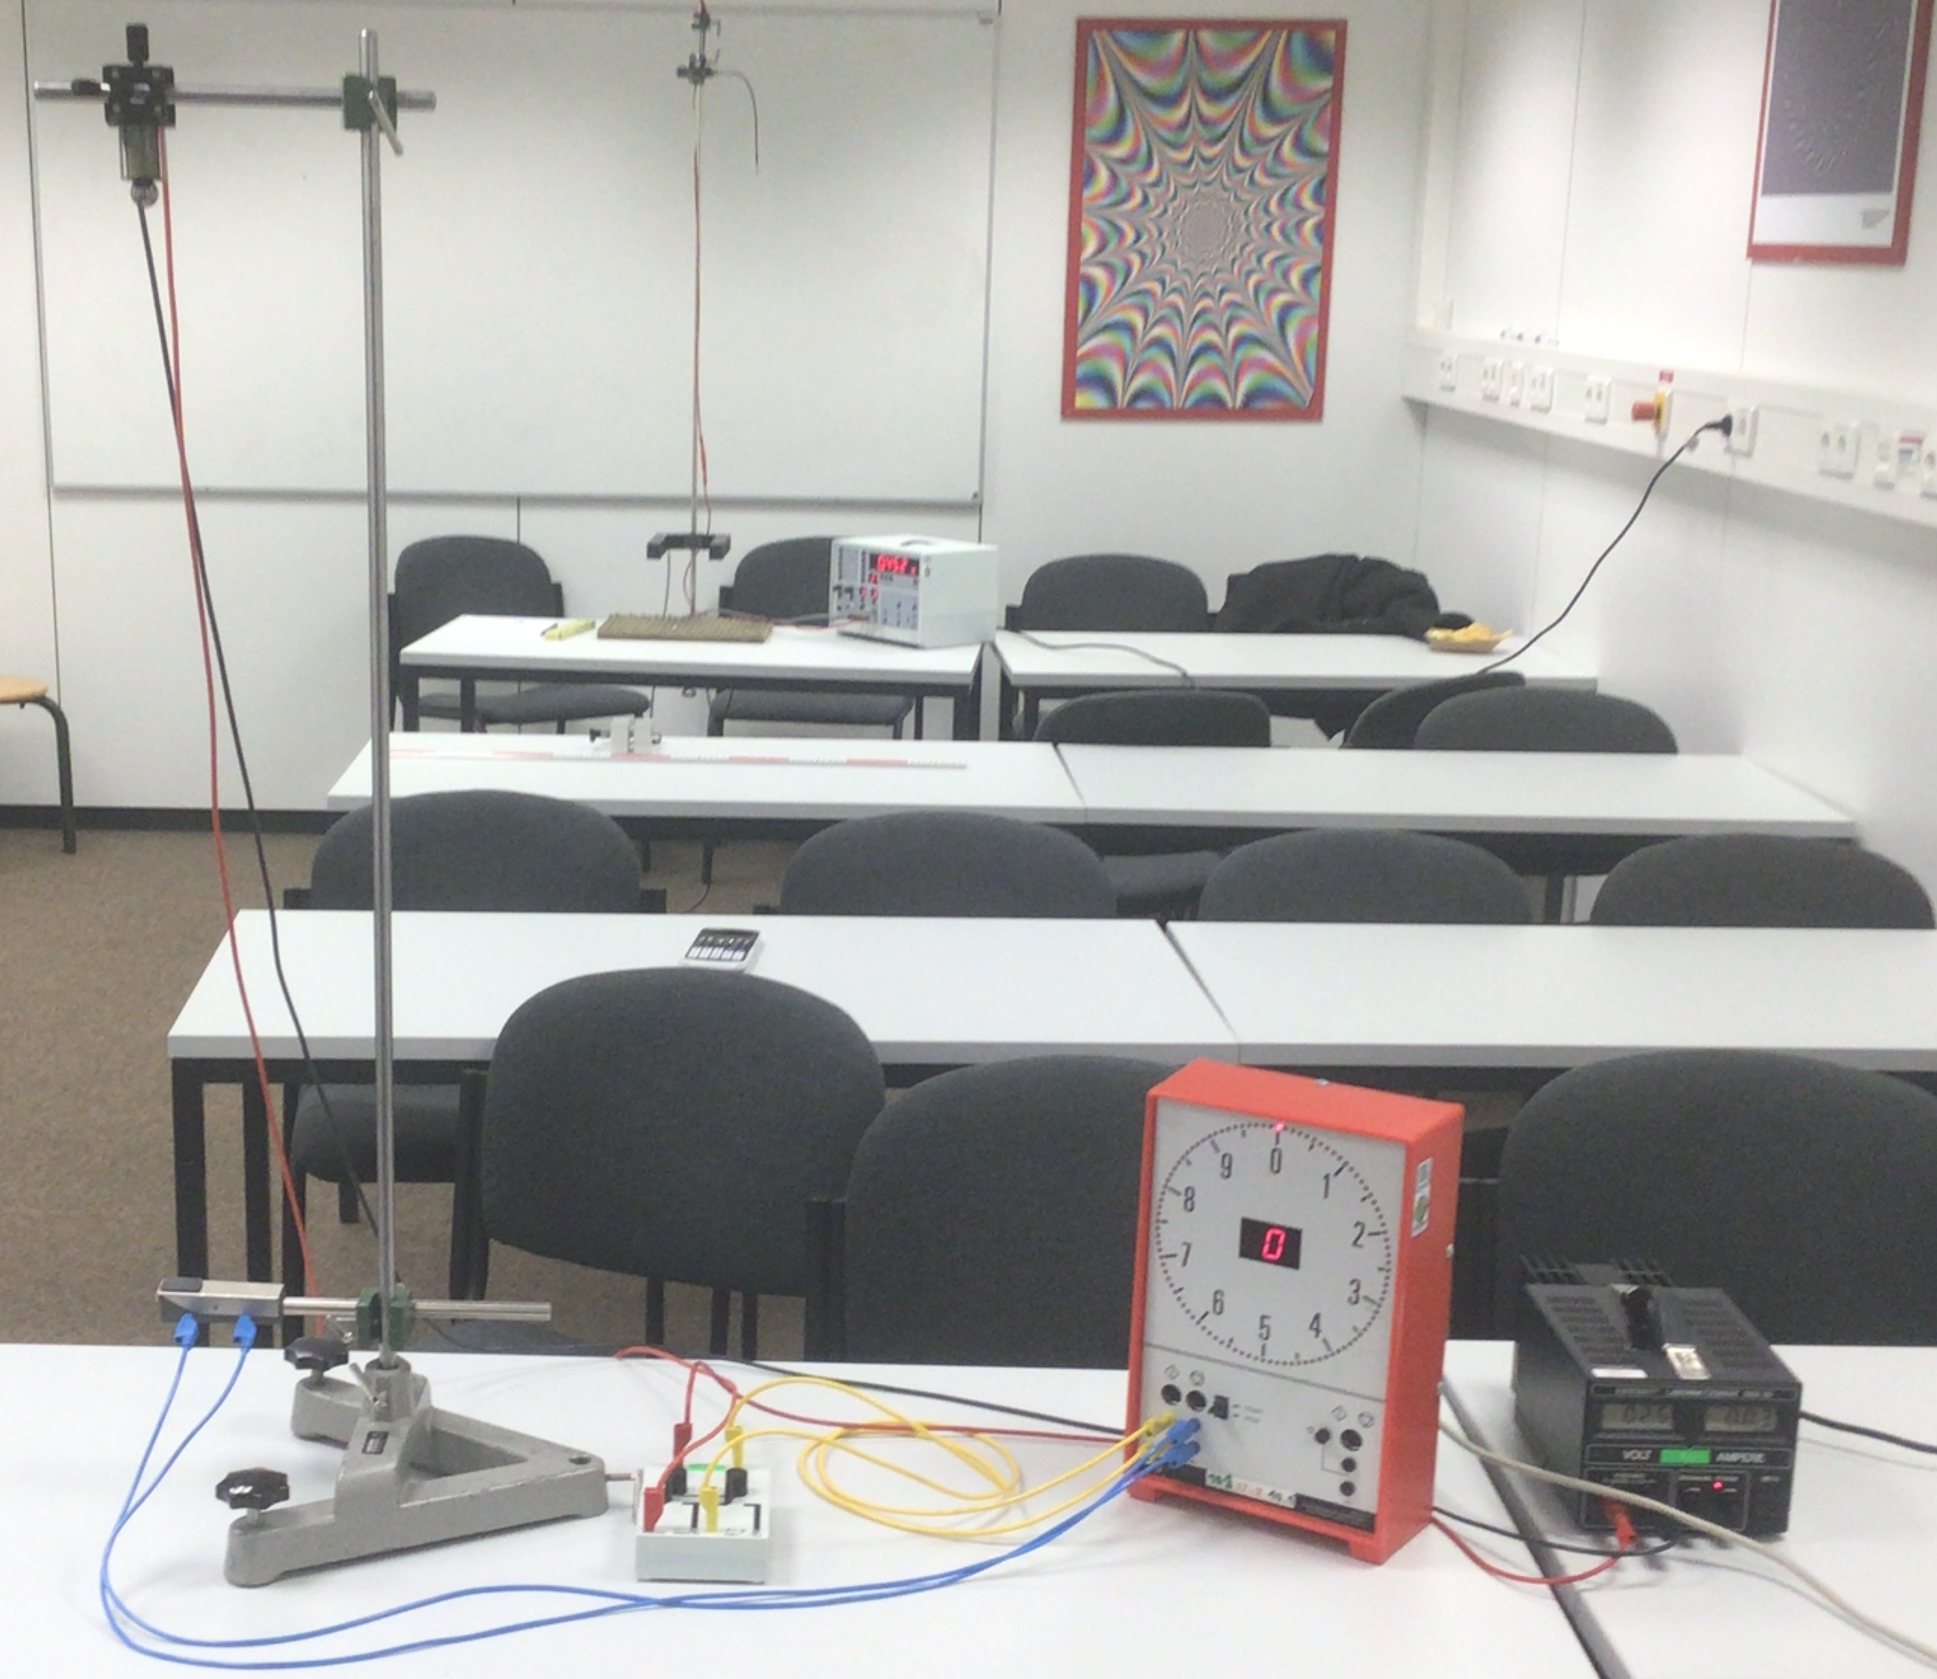
\includegraphics[width=0.75\textwidth]{img/versuchsaufbau}
    \end{minipage}

    \vspace{0.5cm}
    \textbf{Aufbau}: Das Experiment besteht aus drei Stromkreisen. In einem versorgt das Netzteil eine Spule (Haltemagnet) mit dem notwendigen Strom um eine Metallkugel zu halten (Kabel rot/schwarz). Dieser Stromkreis kann durch Umlegen des Schalters getrennt werden. Die anderen beiden liefern Start-und Stoppsignal (Trennen oder Schließen) für das Zählgerät. Das Startsignal wird durch Umlegen des Schalters (Kabel gelb) verursacht. Das Stoppsignal erfolgt durch Herunterdrücken der Metallplatte (Kabel blau).
    
    \vspace{0.5cm}
    \textbf{Durchführung}: Zu Beginn des Versuchs, schließt der Schalter den Stromkreis des Haltemagneten. Mit dem Maßstab wird dann der Abstand $h$ \glqq Unterkante  Metallkugel\grqq{} zu \glqq Kontaktplatte im geschlossenen Zustand\grqq{} gemessen. Der Schalter wird umgelegt und es beginnt der freie Fall der Metallkugel. Gleichzeitig startet das Zählgerät. Bei Kontakt mit der Metallplatte wird das Stoppsignal ausgelöst und die vergangene Zeit $t$ kann am Zählgerät abgelesen werden.  

    \vspace{0.5cm}
    \textbf{Ergebnis}: Über die Formel
    \begin{align*}
        g(h,t) = \frac{2 \cdot h}{t^2}
    \end{align*}
    lässt sich dann die Fallbeschleunigung im Bereich von $g=9.81 \,\, \frac{\text{m}}{\text{s}^2}$ bestimmen. 
    
    \vspace{0.5cm}
    \textbf{Didaktische Bemerkungen}: Das Experiment bietet sich als Bestätigung von Schülerexperimenten an. Außerdem lässt sich der Versuch durch den Haltemagneten mit unterschiedlischsten Massen durchführen ohne das ein großer Aufwand beim Austauschen entsteht.

    \vspace{0.5cm}
    \textbf{Bemerkungen}: Bei einigen Schaltern ist es sinnvoll, das Startsignal durch Trennen des Stromkreises auszulösen, da die Schalter ansonsten eine leichte Verzögerung aufweisen.

    \vspace{0cm}
\end{tcolorbox}

\end{document}
